\chapter{背景与相关工作}\label{background}

GPU编程已经成为了科学计算和深度学习等领域的重要手段,其中CUDA是最流行的GPU编程语言之一。相比于CPU,GPU执行模型的主要差异在于它具有数千个处理器核心,能够以极高的并行度执行任务。要想充分利用GPU的计算能力及理解本文提出的ko-Sched框架,读者需要了解一些基础概念、调度算法以及核心分割技术等相关知识。

在本章节,我们将介绍CUDA编程中的基础概念,NVIDIA GPU的调度算法及CUDA编程中使用的核心分割技术。

\section{CUDA编程基础}

CUDA是英伟达公司开发的用于通用并行计算平台和编程模型,它可以利用GPU进行计算加速。CUDA编程涉及到两个主要部分:在主机(CPU)上运行的主机代码和在设备(GPU)上运行的设备代码。主机代码负责初始化设备、管理内存、启动设备代码并从设备中获取结果。一个典型CUDA程序包括以下部分:
\begin{enumerate*}[label=\roman*),itemjoin={\quad}]
    \item 在GPU显存中分配空间:程序首先需要在设备上分配内存,以便在设备上运行内核。这可以通过使用CUDA库函数\texttt{cudaMalloc()}实现。
    \item 将数据从主机内存复制到设备内存:在设备可以使用数据之前,主机需要先初始化内核使用的输入数据。这可以通过使用CUDA库函数\texttt{cudaMemcpy()}实现。
    \item 启动设备代码:设备代码是使用CUDA编写的代码,它会在设备上并行运行。内核是一组并行运行的线程,每个线程独立地执行设备代码的一部分。启动设备代码需要使用CUDA库函数\texttt{<<<>>>}运算符和kernel函数名称。
    \item 将数据从设备内存复制回主机内存:在内核运行完毕后,将数据从设备内存复制回主机内存,从而主机可使用设备计算的结果。这可以通过使用CUDA库函数\texttt{cudaMemcpy()}实现。
    \item 释放设备内存:最后,程序需要在设备上释放使用的内存。这可以通过使用CUDA库函数\texttt{cudaFree()}实现。
\end{enumerate*}。

这些操作被抽象为\emph{复制}和\emph{执行}命令,并被存储在GPU调度队列中,分别由\emph{CE}(Copy engine)和\emph{EE}(Execution engine)执行。当输入数据被复制至GPU显存后,CUDA编程模型以\emph{单指令多线程}(Single Intruction Multiple Threads, SIMT)的方式执行内核,多个线程对不同的数据执行同样的指令。同一个block中的线程在逻辑上被划分为若干大小为32的组,称为\emph{warp},每个warp中的线程会并行执行同样的指令。Warp是GPU中最小调度单元。

除了warp外,CUDA编程还引入了其他层次的并行结构。一个kernel通常由单个grid构成,grid由若干block构成,而block包括一系列可以并行的warp。GPU设备由若干\emph{流处理器}(SM)组成,每个流处理器内的warp调度模块负责将warp分配给可用的硬件资源。当kernel从调度列表中被派发时,block调度模块将其中每个block分配到一个SM中,直至所有block均被分配或没有足够的可用硬件资源。Grid和block均可组织为1维、2维或3维。当block被分配到硬件时,其维度信息将被消除而仅视为一系列warp。

\begin{lstlisting}[language=C++, label=code:naivehostcudacode, caption=Host code for naive matrix transpose, float, firstnumber=1, escapeinside={(*}{*)}]
void cpuThread() {
    // data init and allocation
    const size_t msize = W_MATRIX*H_MATRIX*sizeof(float);
    float *h_iData = (float*)malloc(msize); (*\label{code:naivehostcudacode:allocbeg}*)
    float *h_oData = (float*)malloc(msize);
    float *d_iData = cudaMalloc(&d_iData,msize);
    float *d_oData = cudaMalloc(&d_oData,msize); (*\label{code:naivehostcudacode:allocend}*)

    fillInputData(h_iData, ...); (*\label{code:naivehostcudacode:initdata}*)
    dim3 dimGrid(W_MATRIX/TILE_DIM, H_MATRIX/TILE_DIM, 1); (*\label{code:naivehostcudacode:configbeg}*)
    dim3 dimBlock(TILE_DIM, BLOCK_ROWS, 1); (*\label{code:naivehostcudacode:configend}*)

    // actual command submission
    cudaMemcpy (d_iData, h_iData, msize, cudaMemcpyHostToDevice); (*\label{code:naivehostcudacode:cpyto}*)
    transpose<<<dimGrid, dimBlock>>>(d_Odata,d_iData); (*\label{code:naivehostcudacode:kernel}*)
    cudaMemcpy (h_oData, d_oData, msize, cudaMemcpyDeviceToHost);
    cudaDeviceSynchronize();
    // data postprocessing
}
\end{lstlisting}

\begin{lstlisting}[language=C++, label=code:naivedevicecudacode, caption=Device code for naive matrix transpose, float, firstnumber=1, escapeinside={(*}{*)}]
__global__ void transpose(float *odata, const float *idata){
    int x = blockIdx.x * TILE_DIM + threadIdx.x; (*\label{code:naivedevicecudacode:idxbeg}*)
    int y = blockIdx.y * TILE_DIM + threadIdx.y; (*\label{code:naivedevicecudacode:idxend}*)
    int width = gridDim.x * TILE_DIM;
    for (int j = 0; j < TILE_DIM; j += BLOCK_ROWS) (*\label{code:naivedevicecudacode:loopbeg}*)
        odata[x * width + (y + j)] = idata[(y + j) * width + x]; (*\label{code:naivedevicecudacode:loopend}*)
}
\end{lstlisting}

\autoref{code:naivehostcudacode}和\autoref{code:naivedevicecudacode}展示了简化的CUDA代码,这段代码转置了由\texttt{float}组成的大小为\texttt{W\_MATRIX\ \times\ H\_MATRIX}的矩阵。\autoref{code:naivehostcudacode}中第一步是为主机和设备数据分配内存(\autoref{code:naivehostcudacode:allocbeg}\textasciitilde\autoref{code:naivehostcudacode:allocend}):对于主机数据,使用常规的\texttt{malloc}函数,而对于设备数据,使用CUDA API runtime函数\texttt{cudaMalloc}。然后初始化主机内存(\autoref{code:naivehostcudacode:initdata}),定义内核启动配置(\autoref{code:naivehostcudacode:configbeg}\textasciitilde\autoref{code:naivehostcudacode:configend})。\texttt{dim3}数据结构包含三个整数值,表示沿$x$、$y$和$z$维的线程或块的数量。矩阵被划分为多个tile,每个block操作该部分矩阵。在本例中,block是二维的,故第三维设置为$1$。\texttt{dimGrid}包含内核的block数目(即矩阵宽度或高度/\texttt{TILE\_DIM}),而\texttt{dimBlock}定义每个块中的线程数(即\texttt{TILE\_DIM\ \times\ BLOCK\_ROWS})。

主机发出复制命令,将数据从主机传输到设备(\autoref{code:naivehostcudacode:cpyto})。\autoref{code:naivehostcudacode:kernel}启动了内核。内核的名称(在本例中为\texttt{transpose})必须与设备代码的函数名一致。

\autoref{code:naivedevicecudacode} 中要注意的是通过线程索引(\autoref{code:naivedevicecudacode:idxbeg}\textasciitilde\autoref{code:naivedevicecudacode:idxend})进行任务划分。通过CUDA关键字\texttt{threadIdx.x/y}检索块内线程ID,通过\texttt{blockId.x/y}检索block的ID,沿$x$维的块数量可以通过\texttt{gridDim.x}关键字查询。基于这些ID,每个工作线程将计算自己的输入/输出数据的索引偏移量。在本例中,\texttt{TILE\_DIM = 32},\texttt{BLOCK\_ROWS = 8},\texttt{iData}和\texttt{oData}均为$ 1024\times 1024 $元素矩阵。\autoref{code:naivedevicecudacode:loopbeg}\textasciitilde\autoref{code:naivedevicecudacode:loopend}的循环告诉我们,块中的每个线程从\texttt{iData}读取4个元素,步幅为$32 \times 8$个元素,并复制至\texttt{oData}对应位置。

CUDA为编程人员提供了使复制和执行操作相交替的操作,这是通过使用\emph{CUDA流}(stream)来实现的。CUDA流是GPU命令队列的抽象,每个复制或执行命令都需要指明其所处的流。如果未指定流,则CUDA运行时使用\emph{默认流}(stream NULL),它会与同一应用程序的其他流进行隐式同步。在不同的流中推送的命令可以交错执行,并且在可能的情况下可以同时运行。同一流中的命令以FIFO方式排序,并且不能重叠。流执行可以是同步或异步的。如果是同步的,则CPU线程将工作分派到GPU并在内核完成之前阻塞。如果是异步的,则在GPU执行期间可以进行CPU计算。在两种情况下,GPU内核完成后,如果CPU或其他计算设备需要,CE会将由GPU计算的结果复制回主机。

\section{NVIDIA GPU 调度算法简介}\label{nvidia-sched}

主机代码启动kernel后,kernel会被加入所在stream的队列。当kernel从调度队列被选中运行时,设备的block调度模块将kernel的每个block分配给1个SM。尽管由于NVIDIA GPU的闭源属性,公开文档中没有详细说明调度策略,但 \citet{8277284}, \citet{9113104}, \citet{8853389}的工作和本文中的实验表明GPU会先将硬件资源分配给当前kernel,若在分配完毕后设备仍有剩余资源则会分配给下一个kernel。

\begin{figure}[htbp]
    \centering
    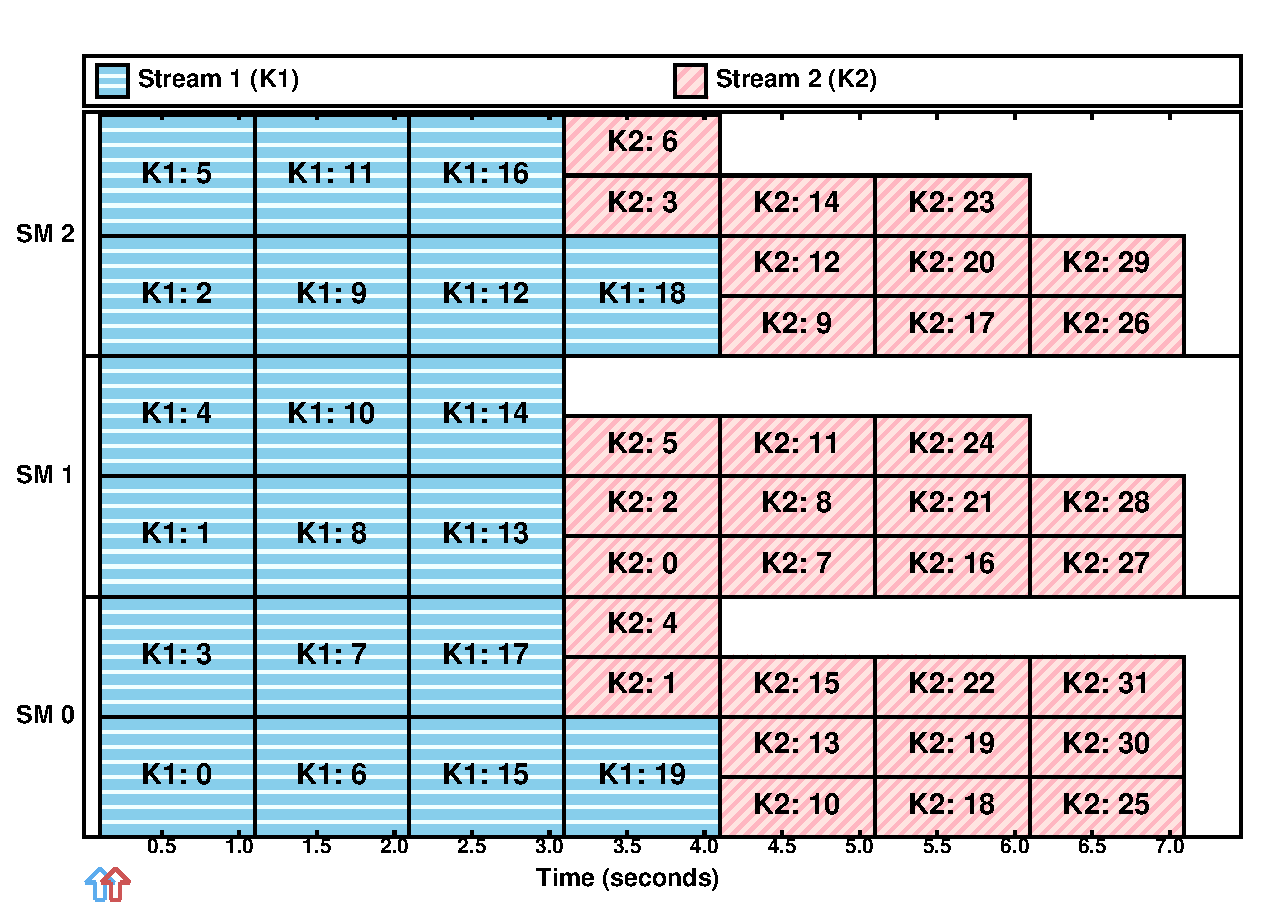
\includegraphics[width=0.9\linewidth]{sm_level_kernel_scheduling/kernel_nonparallel.pdf}
    \caption{kernel启动后每个SM的block分配情况。}
    \label{sm-level-kernel-scheduling}
\end{figure}

\begin{figure}[htbp]
    \centering
    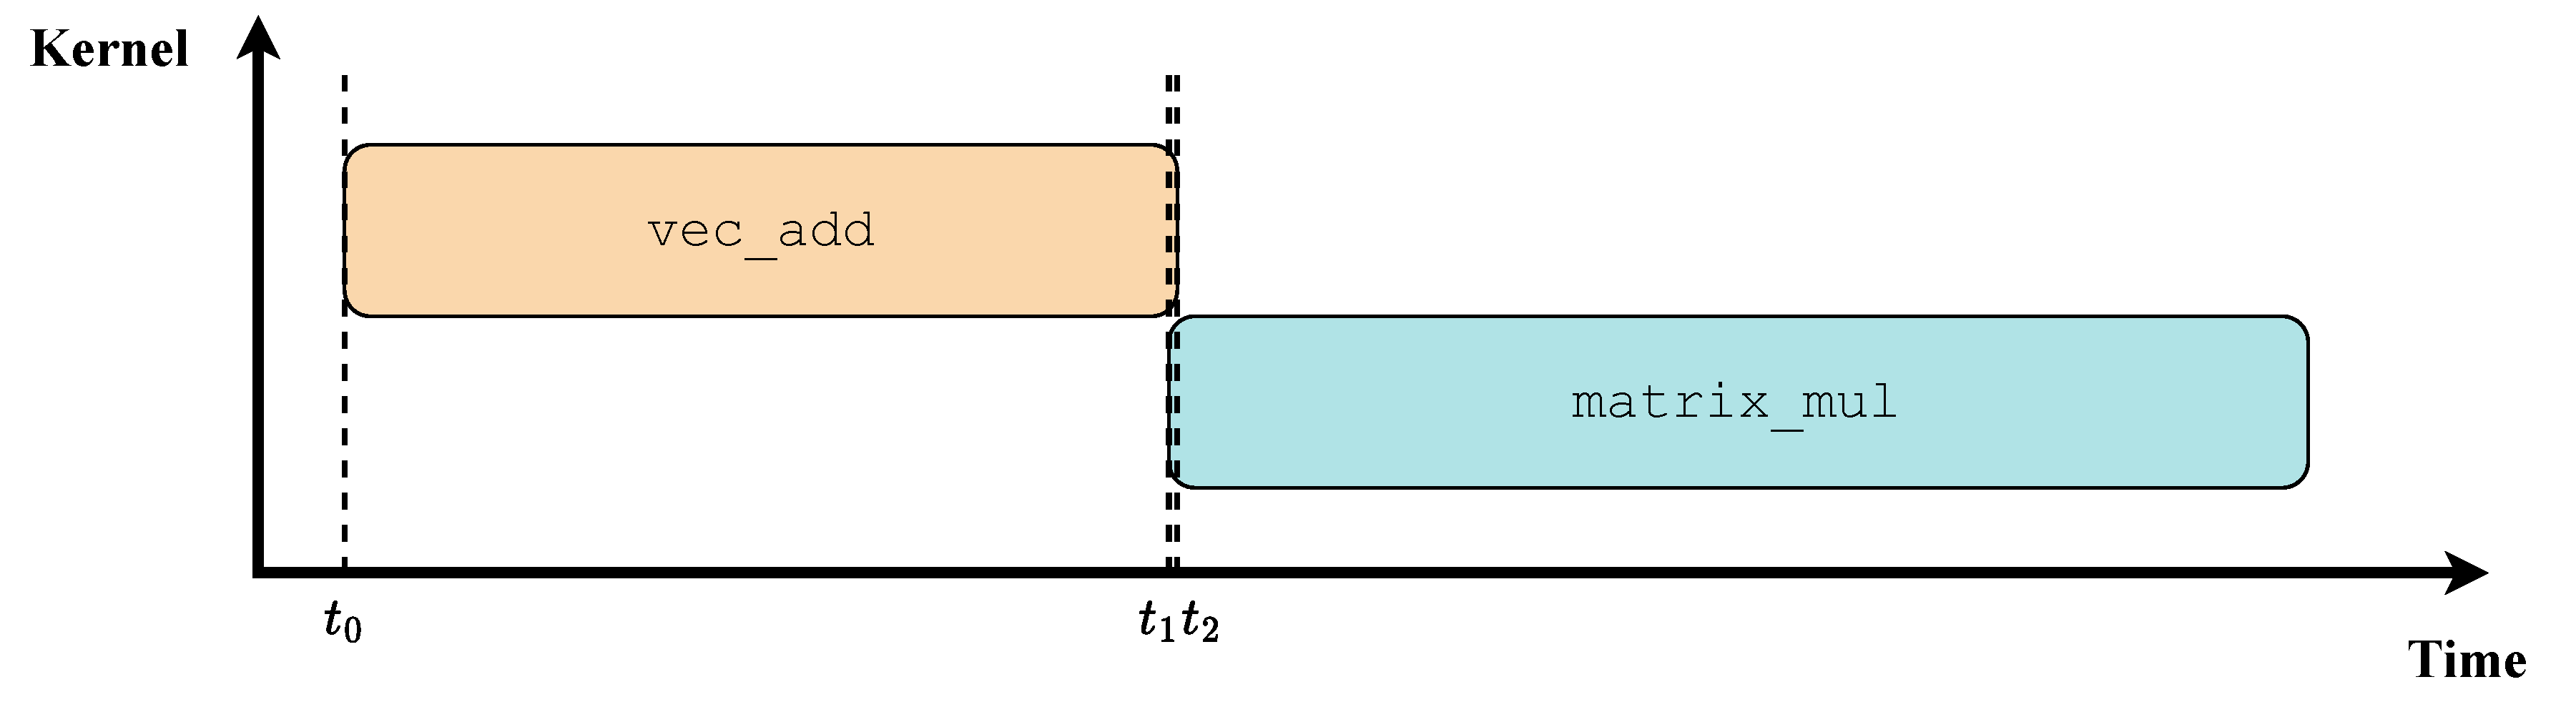
\includegraphics[width=0.9\linewidth]{va_mm_serial/serial_execution.drawio.pdf}
    \caption{kernel执行的时间轴}
    \label{serial-execution}
\end{figure}

为具体展示此策略,我们使用CUDA scheduling mirror\cite{otterness2017inferring}分析一个程序中block的分配情况。为简化分析,我们选择了SM数目较少的NVIDA GeForce MX250运行此实验\footnote{对于此运行环境的具体介绍见\autoref{evaluation}\autoref{exp-env}。}。我们先后在不同的stream中启动内核$K_1$, $K_2$,如\autoref{sm-level-kernel-scheduling}所示,每一个矩形代表了一个block: $K_i$的第$j$个block被标记为$Ki:j$,矩形的左右边界表示了block执行的开始与结束时间(通过GPU的\texttt{globaltimer}寄存器记录),矩形的高度表示了此block所拥有的thread数目,矩阵在垂直方向的位置表明了它被分配至的SM,$x$轴下方的箭头表示了kernel启动的时间。可见,内核$K_1$, $K_2$从不同stream启动后,$K_1$的block 0\textasciitilde 5被分配至SM 0\textasciitilde 2。此时,由于设备的剩余资源无法满足$K_1$的下一个block,直至block 0\textasciitilde 5执行完毕后$K_1$的剩余block才被分配至GPU。当$K_1$的block 18\textasciitilde 19被分配至SM后,由于GPU仍有剩余资源,调度模块将$K_2$的block分配给空闲的SM。

此策略带来的影响为,若不做特殊处理,2个kernel一般并不会并行执行。我们使用Nsight Systems\cite{nsightsystems}查看kernel执行的时间线。以\texttt{vec\_add}和\texttt{matrix\_mul}\footnote{关于本文用到的测试程序的详细信息,见\autoref{evaluation}\autoref{exp-env}}为例,如\autoref{serial-execution}所示,$t_0$时刻2个kernel从不同stream先后启动。\texttt{vec\_add}在$t_0$至$t_2$时刻运行,\texttt{matrix\_mul}从$t_1$时刻开始运行。$t_1$至$t_2$时段2个kernel在并行执行。可见,尽管2个kernel从不同的stream启动,它们只有很短的时间内在并行执行。

\section{内核分割}

\citet{10.1145_3295690}\cite{8853389}的研究表明,使不同类型的kernel并行运行可能实现性能提升。例如,计算密集型kernel和内存密集型kernel并行可提高GPU硬件的利用率,从而降低总执行时间。然而,GPU的调度策略给kernel的并行带来困难。\autoref{serial-execution}中的例子说明,若不做其他处理,简单地使用stream难以实现kernel并行带来的性能提升。

为使不同kernel能并行执行,开发者可以使用\emph{内核分割技术}(kernel slicing),即,将kernel包含的block划分为若干组,每组形成1个\emph{子内核}(sub-kernel)。将同属于1个内核的子内核在同一stream内顺序启动。由于单个子内核占用资源较少,子内核开始执行后设备仍有资源执行其他内核的子内核,从而实现了kernel的并行。

由于涉及到将kernel分割及不同kernel的并行,内核分割对kernel的特性有特别的约束:
\begin{enumerate}
    \item Kernel间无数据依赖
    \item Kernel的计算不依赖于grid的维度、大小
    \item Kernel的控制流不依赖于数据。否则,若部分线程的行为因输入数据不同而显著异于其他线程,可能会间接导致分割后的子内核特性相异,进而使性能未达到预期提升
    \item Kernel对设备cache大小相对不敏感。否则,不同kernel并行时对设备cache有抢占行为,会影响某些kernel性能
\end{enumerate}

本文中实验所用到的测试程序均满足以上假设。

\begin{figure}[htbp]
    \centering
    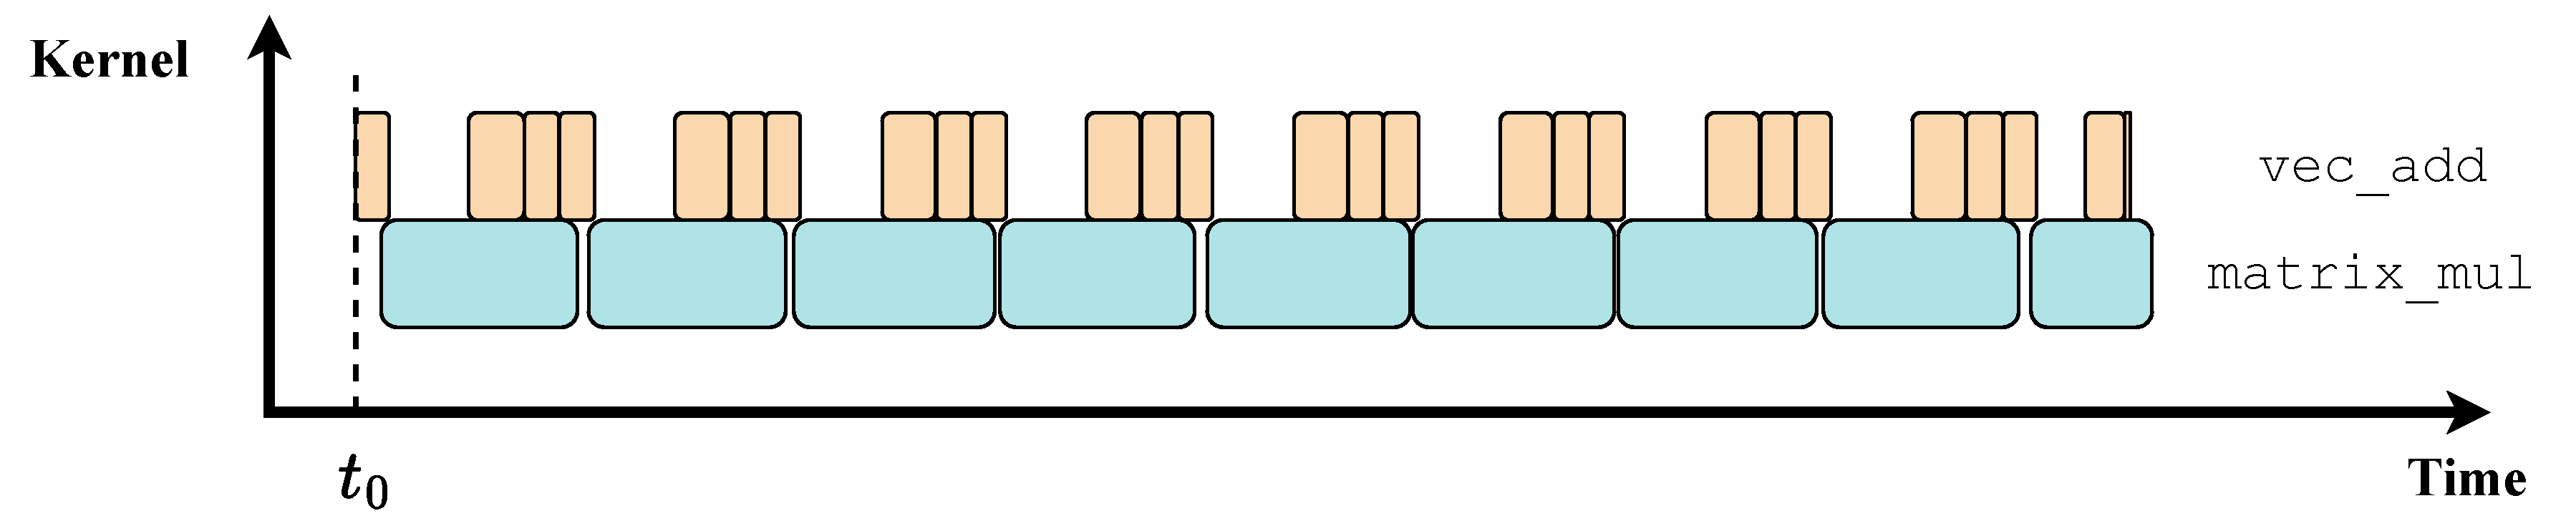
\includegraphics[width=0.9\linewidth]{opt_cosched/opt_cosched.drawio.pdf}
    \caption{内核分割技术的并行执行}
    \label{opt-cosched}    
\end{figure}

\autoref{opt-cosched}展示了\texttt{vec\_add}和\texttt{matrix\_mul}在使用内核分割技术后并行执行的时间线。$t_0$时刻,这2个内核的所有子内核在2个stream中启动,进入stream对应的调度队列。之后,调度模块从队列中选择可执行的内核派发至执行单元。由于单个子内核block数目较少,在分配后GPU仍有剩余资源,调度模块可选择其他子内核同时执行。

\section{相关工作}

本节介绍GPU协同调度的相关工作。在GPU调度的广泛背景下,存在以下多方面的相关工作:

\citet{6777559}和\citet{7802143}介绍了软件仿真框架,将内核转换为设备函数,较大的内核会调用较小的设备函数以利用SM共享,并用动态规划求出解决方案。\citet{6624111}提出一种内核分块方案,以防止单个内核占用所有SM资源,而\citet{10.1145/2451116.2451160}的工作则考虑资源可用性以动态调整内核大小。\citet{10.1145/2751205.2751213}提出了一种SM中心的程序代码转换方法,通过将任务和线程之间的绑定替换为任务和SM之间的绑定来实现。

有些工作关注于在单GPU环境中采用不同的方法。有些考虑修改GPU架构,如warp调度器、寄存器文件或内存控制子系统,而有些则需要在驱动程序或编译器中进行更改。SMK\cite{7446078}尝试使用“Dominant Resource Fairness”这一标准公平地分配内核之间的静态资源。它还利用性能分析器在运行时分配warp指令的配额。Warped-Slicer\cite{10.1109/ISCA.2016.29}提出了一种以最小开销将内核的线程块划分为与其他内核并发执行的部分的方法。\citet{8327010}平衡了并发内核的内存访问,并限制正在进行的内存指令的数量,以克服L1缓存抖动和内存流水线停顿的问题。Leano等人介绍了schedGPU\cite{8219713},这是一种客户端-服务器和共享内存方法,用于同步多个内核对GPU的访问。cCUDA\cite{8853389}通过选取合适的指标将内核分类为计算密集型和内存密集型,并将不同类型内核配对联合调度以提高GPU资源利用。

除了软件方法之外,还有像\citet{10.1145/3007787.3001161}和\citet{8310677}的方法,提出了对设备组件(如warp调度程序和GigaThread调度程序)的硬件修改。

Ko-Sched在软件层面上实现了离线的协同调度,通过将内核分割为子内核,使不同类型的内核能并行执行。Ko-Sched的优势在于,不需要修改GPU硬件,也不需要修改GPU驱动程序或编译器。Ko-Sched的缺点在于,它假设了同一内核的分片是等大小的,不会在运行时动态改变,且分割后的子内核的特性可能不同,从而可能导致性能未达到预期提升。
